\documentclass{uofa-eng-assignment}
\usepackage{pythonhighlight}
\usepackage{float}
\usepackage{amsmath}
\usepackage{enumerate}% http://ctan.org/pkg/enumerate
\usepackage{lipsum, afterpage}
\usepackage{hyperref}
\usepackage{amsmath, amsthm, amssymb, amsfonts, physics}
\usepackage{mathtools}
\usepackage{graphicx}
\usepackage{fdsymbol}
\usepackage{xcolor}

\hypersetup{
    colorlinks=true,
    linkcolor=blue,
    filecolor=magenta,
    urlcolor=cyan,
    pdftitle={Overleaf Example},
    pdfpagemode=FullScreen,
}

\graphicspath{ {./images/} }

\DeclareRobustCommand{\rchi}{{\mathpalette\irchi\relax}}
\newcommand{\infdiv}{D\infdivx}
\newcommand{\irchi}[2]{\raisebox{\depth}{$#1\chi$}} % inner command, used by \rchi
\newcommand\aug{\fboxsep=-\fboxrule\!\!\!\fbox{\strut}\!\!\!}
\newcommand*{\name}{\textbf{Luke Nguyen}}
\newcommand*{\id}{\textbf{D5850A}}
\newcommand*{\course}{Statistical Methods and Data Analysis (EN.625.603)}
\newcommand*{\assignment}{Final Exam}

\begin{document} \maketitle
%%%%%%%%%%%%%%%%%%%%%%%%%%%%%%%%%%%%%%%%%%%%%%%%%%%%%%%%%%%%%%%%%%%%%%%%%%%%%%%%%%%%%%%%%%%%%%%%%%%%    
Description: The datafile contains data for 2015 for full-time workers with a
high school diploma or B.A./B.S. as their highest degree. See the pdf
attachment for an overview of the data and variable descriptions. In this
exercise, you will investigate the relationship between a worker's age and
earnings. (Generally, older workers have more job experience, leading to higher
productivity and higher earnings.)

\begin{enumerate}
    %%%%%%%%%%%%%%%%%%%%%%%%%%%%%%%%%%%%%%%%%%%%%%%%%%%%%%%%%%%%%%%%%%%%%%%%%%%%%%%%%%%%%%%%%%%%%%%%%%%%    
    %%%%%%%%%%%%%%%%%%%%%%%%%%%%%%%%%%%%%%%%%%%%%%%%%%%%%%%%%%%%%%%%%%%%%%%%%%%%%%%%%%%%%%%%%%%%%%%%%%%%    
    %%%%%%%%%%%%%%%%%%%%%%%%%%%%%%%%%%%%%%%%%%%%%%%%%%%%%%%%%%%%%%%%%%%%%%%%%%%%%%%%%%%%%%%%%%%%%%%%%%%%    
    %%%%%%%%%%%%%%%%%%%%%%%%%%%%%%%%%%%%%%%%%%%%%%%%%%%%%%%%%%%%%%%%%%%%%%%%%%%%%%%%%%%%%%%%%%%%%%%%%%%%    
    %%%%%%%%%%%%%%%%%%%%%%%%%%%%%%%%%%%%%%%%%%%%%%%%%%%%%%%%%%%%%%%%%%%%%%%%%%%%%%%%%%%%%%%%%%%%%%%%%%%%    
    \item[a.] Run a regression of average hourly earnings $(AHE)$ on $age$ ($Age$),
        $gender$ ($Female$), and $education$ ($Bachelor$). If $age$ increases from 25
        to 26, how are earnings expected to change? If $age$ increases from 33 to 34,
        how are earnings expected to change? \\ \textbf{Solution:} \\ Running
        regression model of $ahe$ on $age, female, bachelor$ in Python yields the
        following results:
        \begin{figure}[H]
            \centering
            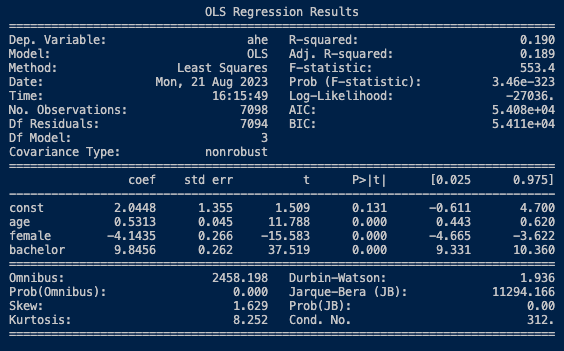
\includegraphics[width=0.80\textwidth]{final-exam-a-1.png}
        \end{figure}
        which is equivalent to the following linear regression equation:
        \begin{align*}
            ahe & = \beta_0 + \beta_1 (age) + \beta_2 (female) + \beta_3 (bachelor) \\
            ahe & = 2.0448 + 0.5313 (age) - 4.1435 (female) + 9.8456 (bachelor)
        \end{align*}
        The coefficient for $age$ is $\beta_1 = 0.5313$.
        This means that for every one unit increase in $age$, $ahe$ is expected to increases by \textbf{$\boldsymbol{0.5313}$ dollars}.
        This applies to both the change from age 25 to 26 and the change from age 33 to 34.\newpage
        %%%%%%%%%%%%%%%%%%%%%%%%%%%%%%%%%%%%%%%%%%%%%%%%%%%%%%%%%%%%%%%%%%%%%%%%%%%%%%%%%%%%%%%%%%%%%%%%%%%%    
        %%%%%%%%%%%%%%%%%%%%%%%%%%%%%%%%%%%%%%%%%%%%%%%%%%%%%%%%%%%%%%%%%%%%%%%%%%%%%%%%%%%%%%%%%%%%%%%%%%%%    
        %%%%%%%%%%%%%%%%%%%%%%%%%%%%%%%%%%%%%%%%%%%%%%%%%%%%%%%%%%%%%%%%%%%%%%%%%%%%%%%%%%%%%%%%%%%%%%%%%%%%    
        %%%%%%%%%%%%%%%%%%%%%%%%%%%%%%%%%%%%%%%%%%%%%%%%%%%%%%%%%%%%%%%%%%%%%%%%%%%%%%%%%%%%%%%%%%%%%%%%%%%%    
        %%%%%%%%%%%%%%%%%%%%%%%%%%%%%%%%%%%%%%%%%%%%%%%%%%%%%%%%%%%%%%%%%%%%%%%%%%%%%%%%%%%%%%%%%%%%%%%%%%%%    
    \item[b.] Run a regression of the logarithm of average hourly earnings, $\ln{(AHE)}$,
        on $Age$, $Female$, and $Bachelor$. If $age$ increases from 25 to 26, how are
        earnings expected to change? If $age$ increases from 33 to 34, how are earnings
        expected to change? \\ \textbf{Solution:} \\ Running regression model of
        $\ln{(ahe)}$ on $age, female, bachelor$ in Python yields the following results:
        \begin{figure}[H]
            \centering
            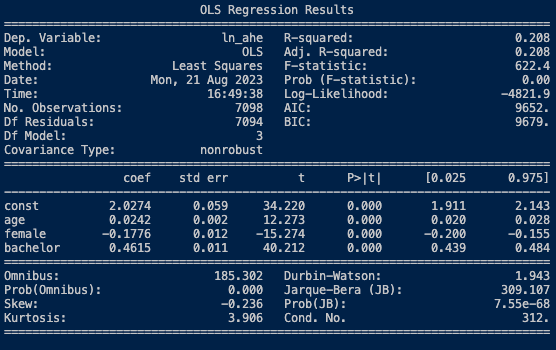
\includegraphics[width=0.80\textwidth]{final-exam-b-1.png}
        \end{figure}
        which is equivalent to the following linear regression equation:
        \begin{align*}
            \ln{(ahe)} & = \beta_0 + \beta_1 (age) + \beta_2 (female) + \beta_3 (bachelor) \\
            \ln{(ahe)} & = 2.0274 + 0.0242 (age) - 0.1776 (female) + 0.4615 (bachelor)
        \end{align*}
        The coefficient for $age$ is $\beta_1 = 0.0242$.
        This means that for every one unit increase in $age$, $\ln{(ahe)}$ is expected to increases by $0.0242$.
        As the model is an exponential model for $ahe$, we can say that for every one unit increase in $age$,
        $ahe$ is expected to increases by $\boldsymbol{2.42\%}$.
        %%%%%%%%%%%%%%%%%%%%%%%%%%%%%%%%%%%%%%%%%%%%%%%%%%%%%%%%%%%%%%%%%%%%%%%%%%%%%%%%%%%%%%%%%%%%%%%%%%%%    
        %%%%%%%%%%%%%%%%%%%%%%%%%%%%%%%%%%%%%%%%%%%%%%%%%%%%%%%%%%%%%%%%%%%%%%%%%%%%%%%%%%%%%%%%%%%%%%%%%%%%    
        %%%%%%%%%%%%%%%%%%%%%%%%%%%%%%%%%%%%%%%%%%%%%%%%%%%%%%%%%%%%%%%%%%%%%%%%%%%%%%%%%%%%%%%%%%%%%%%%%%%%    
        %%%%%%%%%%%%%%%%%%%%%%%%%%%%%%%%%%%%%%%%%%%%%%%%%%%%%%%%%%%%%%%%%%%%%%%%%%%%%%%%%%%%%%%%%%%%%%%%%%%%    
        %%%%%%%%%%%%%%%%%%%%%%%%%%%%%%%%%%%%%%%%%%%%%%%%%%%%%%%%%%%%%%%%%%%%%%%%%%%%%%%%%%%%%%%%%%%%%%%%%%%%
    \item[c.] Run a regression of the logarithm of average hourly earnings, $ln(AHE)$, on
        $ln(Age)$, $Female$, and $Bachelor$. If $age$ increases from 25 to 26, how are
        earnings expected to change? If $age$ increases from 33 to 34, how are earnings
        expected to change? \newpage \textbf{Solution:} \\ Running regression model of
        $ln(ahe)$ on $ln(age), female, bachelor$ in Python yields the following
        results:
        \begin{figure}[H]
            \centering
            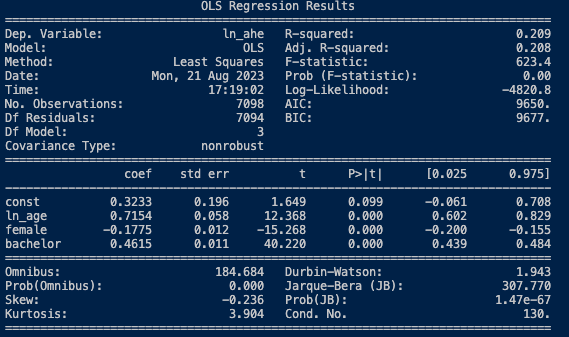
\includegraphics[width=0.80\textwidth]{final-exam-c-1.png}
        \end{figure}
        which is equivalent to the following linear regression equation:
        \begin{align*}
            \ln{(ahe)} & = \beta_0 + \beta_1 (\ln{(age)}) + \beta_2 (female) + \beta_3 (bachelor) \\
            \ln{(ahe)} & = 0.3233 + 0.7154 (\ln{(age)}) - 0.1775 (female) + 0.4615 (bachelor)
        \end{align*}
        The coefficient for $\ln{(age)}$ is $\beta_1 = 0.7154$. \\
        For age increases from 25 to 26, age increases by $\frac{26 - 25}{25} = 4\%$, thus $\ln{(ahe)}$ is expected to increases by $0.7154 \times 4\% = \boldsymbol{2.8616\%}$. \\
        For age increases from 33 to 34, age increases by $\frac{34 - 33}{33} = 3.03\%$, thus $\ln{(ahe)}$ is expected to increases by $0.7154 \times 3.03\% = \boldsymbol{2.1679\%}$. \\
        %%%%%%%%%%%%%%%%%%%%%%%%%%%%%%%%%%%%%%%%%%%%%%%%%%%%%%%%%%%%%%%%%%%%%%%%%%%%%%%%%%%%%%%%%%%%%%%%%%%%    
        %%%%%%%%%%%%%%%%%%%%%%%%%%%%%%%%%%%%%%%%%%%%%%%%%%%%%%%%%%%%%%%%%%%%%%%%%%%%%%%%%%%%%%%%%%%%%%%%%%%%    
        %%%%%%%%%%%%%%%%%%%%%%%%%%%%%%%%%%%%%%%%%%%%%%%%%%%%%%%%%%%%%%%%%%%%%%%%%%%%%%%%%%%%%%%%%%%%%%%%%%%%    
        %%%%%%%%%%%%%%%%%%%%%%%%%%%%%%%%%%%%%%%%%%%%%%%%%%%%%%%%%%%%%%%%%%%%%%%%%%%%%%%%%%%%%%%%%%%%%%%%%%%%    
        %%%%%%%%%%%%%%%%%%%%%%%%%%%%%%%%%%%%%%%%%%%%%%%%%%%%%%%%%%%%%%%%%%%%%%%%%%%%%%%%%%%%%%%%%%%%%%%%%%%%
    \item[d.] Run a regression of the logarithm of average hourly earnings, $\ln{(AHE)}$,
        on $Age$, $Age^2$, $Female$, and $Bachelor$. If $age$ increases from 25 to 26,
        how are earnings expected to change? If $age$ increases from 33 to 34, how are
        earnings expected to change? \newpage \textbf{Solution:} \\ Running regression
        model of $\ln{(ahe)}$ on $age, (age^2), female, bachelor$ in Python yields the
        following results:
        \begin{figure}[H]
            \centering
            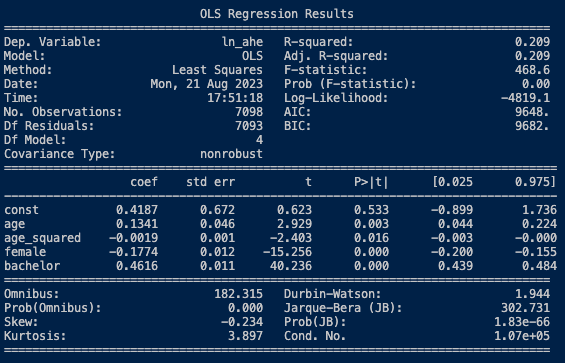
\includegraphics[width=0.80\textwidth]{final-exam-d-1.png}
        \end{figure}
        which is equivalent to the following linear regression equation:
        \begin{align*}
            \ln{(ahe)} & = \beta_0 + \beta_1 (age) + \beta_2 (age^2) + \beta_3 (female) + \beta_4 (bachelor) \\
            \ln{(ahe)} & = 0.4187 + 0.1341 (age) - 0.0019 (age^2) - 0.1774(female) + 0.4616 (bachelor)
        \end{align*}
        The coefficient for $age$ is $\beta_1 = 0.1341$. and the coefficient for $age^2$ is $\beta_2 = -0.0019$. \\
        For age increases from 25 to 26, age increases by
        \begin{align*}
            0.1341 - 0.0019 \times(26^2-25^2) = 3.72\%
        \end{align*}
        thus, $ahe$ is expected to increases by
        \begin{align*}
            \boldsymbol{3.72\%}
        \end{align*}
        For age increases from 33 to 34, age increases by
        \begin{align*}
            0.1341 - 0.0019 \times(34^2-33^2) = 0.68\%
        \end{align*}
        thus, $ahe$ is expected to increases by
        \begin{align*}
            \boldsymbol{0.68\%}
        \end{align*}
        %%%%%%%%%%%%%%%%%%%%%%%%%%%%%%%%%%%%%%%%%%%%%%%%%%%%%%%%%%%%%%%%%%%%%%%%%%%%%%%%%%%%%%%%%%%%%%%%%%%%    
        %%%%%%%%%%%%%%%%%%%%%%%%%%%%%%%%%%%%%%%%%%%%%%%%%%%%%%%%%%%%%%%%%%%%%%%%%%%%%%%%%%%%%%%%%%%%%%%%%%%%    
        %%%%%%%%%%%%%%%%%%%%%%%%%%%%%%%%%%%%%%%%%%%%%%%%%%%%%%%%%%%%%%%%%%%%%%%%%%%%%%%%%%%%%%%%%%%%%%%%%%%%    
        %%%%%%%%%%%%%%%%%%%%%%%%%%%%%%%%%%%%%%%%%%%%%%%%%%%%%%%%%%%%%%%%%%%%%%%%%%%%%%%%%%%%%%%%%%%%%%%%%%%%    
        %%%%%%%%%%%%%%%%%%%%%%%%%%%%%%%%%%%%%%%%%%%%%%%%%%%%%%%%%%%%%%%%%%%%%%%%%%%%%%%%%%%%%%%%%%%%%%%%%%%%
    \item[e.] Do you prefer the regression in (c) to the regression in (b)? Explain.
        \newpage \textbf{Solution:} \\ The model in (c) is a better model than the
        model in (b). \\ Although the $R-squared, Adj. R-squared, AIC, BIC, p-value$ of
        the model (b) and (c) are very close. \\ The model (b) is a linear model for
        the change in the percentage of $ahe$ with respect to the change in $age$, and
        it is fixed at $\boldsymbol{2.42\%}$ for every one unit increase in $age$. \\
        However, in the case of comparing the change in $ahe$ with respect to the
        change in $age$, the model should account for the diminishing return of $ahe$
        with respect to the increase in $age$, as the workers's average hour earnings
        should plateau at some point, for example, between 25 and 26, the increase in
        $ahe$ is $\boldsymbol{2.8616\%}$, but between 33 and 34, the increase in $ahe$
        is only $\boldsymbol{2.1679\%}$, which will be more accurately modeled by the
        model in (c). \\
        %%%%%%%%%%%%%%%%%%%%%%%%%%%%%%%%%%%%%%%%%%%%%%%%%%%%%%%%%%%%%%%%%%%%%%%%%%%%%%%%%%%%%%%%%%%%%%%%%%%%    
        %%%%%%%%%%%%%%%%%%%%%%%%%%%%%%%%%%%%%%%%%%%%%%%%%%%%%%%%%%%%%%%%%%%%%%%%%%%%%%%%%%%%%%%%%%%%%%%%%%%%    
        %%%%%%%%%%%%%%%%%%%%%%%%%%%%%%%%%%%%%%%%%%%%%%%%%%%%%%%%%%%%%%%%%%%%%%%%%%%%%%%%%%%%%%%%%%%%%%%%%%%%    
        %%%%%%%%%%%%%%%%%%%%%%%%%%%%%%%%%%%%%%%%%%%%%%%%%%%%%%%%%%%%%%%%%%%%%%%%%%%%%%%%%%%%%%%%%%%%%%%%%%%%    
        %%%%%%%%%%%%%%%%%%%%%%%%%%%%%%%%%%%%%%%%%%%%%%%%%%%%%%%%%%%%%%%%%%%%%%%%%%%%%%%%%%%%%%%%%%%%%%%%%%%%
    \item[f.] Do you prefer the regression in (d) to the regression in (b)? Explain. \\
        \textbf{Solution:} \\ The model in (d) is a better model than the model in (b).
        \\ We can use the same argument as in (e) to explain why the model in (d) is
        better than the model in (b) as the model in (d) accounts for the diminishing
        return of $ahe$ with respect to the increase in $age$.
        %%%%%%%%%%%%%%%%%%%%%%%%%%%%%%%%%%%%%%%%%%%%%%%%%%%%%%%%%%%%%%%%%%%%%%%%%%%%%%%%%%%%%%%%%%%%%%%%%%%%    
        %%%%%%%%%%%%%%%%%%%%%%%%%%%%%%%%%%%%%%%%%%%%%%%%%%%%%%%%%%%%%%%%%%%%%%%%%%%%%%%%%%%%%%%%%%%%%%%%%%%%    
        %%%%%%%%%%%%%%%%%%%%%%%%%%%%%%%%%%%%%%%%%%%%%%%%%%%%%%%%%%%%%%%%%%%%%%%%%%%%%%%%%%%%%%%%%%%%%%%%%%%%    
        %%%%%%%%%%%%%%%%%%%%%%%%%%%%%%%%%%%%%%%%%%%%%%%%%%%%%%%%%%%%%%%%%%%%%%%%%%%%%%%%%%%%%%%%%%%%%%%%%%%%    
        %%%%%%%%%%%%%%%%%%%%%%%%%%%%%%%%%%%%%%%%%%%%%%%%%%%%%%%%%%%%%%%%%%%%%%%%%%%%%%%%%%%%%%%%%%%%%%%%%%%%
    \item[g.] Do you prefer the regression in (d) to the regression in (c)? Explain. \\
        \textbf{Solution:} \\ The model in (d) is a better model than the model in (c).
        \\ Although, both models in (c) and (d) account for the diminishing return of
        $ahe$ with respect to the increase in $age$, model (d) includes the quadratic
        term of $age$ and its coefficient is negative, thus it represents that after
        passing a certain age, the $ahe$ will decrease with respect to the increase in
        $age$. Which I think is more realistic in the real world. Additionally, the
        increase in $ahe$ with respect to the increase in $age$ is more aggressive in
        early career which also seems to be more accurate. \\ This assumption is more
        of my personal and relative opinion than an absolute proof.
        %%%%%%%%%%%%%%%%%%%%%%%%%%%%%%%%%%%%%%%%%%%%%%%%%%%%%%%%%%%%%%%%%%%%%%%%%%%%%%%%%%%%%%%%%%%%%%%%%%%%    
        %%%%%%%%%%%%%%%%%%%%%%%%%%%%%%%%%%%%%%%%%%%%%%%%%%%%%%%%%%%%%%%%%%%%%%%%%%%%%%%%%%%%%%%%%%%%%%%%%%%%    
        %%%%%%%%%%%%%%%%%%%%%%%%%%%%%%%%%%%%%%%%%%%%%%%%%%%%%%%%%%%%%%%%%%%%%%%%%%%%%%%%%%%%%%%%%%%%%%%%%%%%    
        %%%%%%%%%%%%%%%%%%%%%%%%%%%%%%%%%%%%%%%%%%%%%%%%%%%%%%%%%%%%%%%%%%%%%%%%%%%%%%%%%%%%%%%%%%%%%%%%%%%%    
        %%%%%%%%%%%%%%%%%%%%%%%%%%%%%%%%%%%%%%%%%%%%%%%%%%%%%%%%%%%%%%%%%%%%%%%%%%%%%%%%%%%%%%%%%%%%%%%%%%%%
    \item [h.] Run a regression of $\ln{(AHE)}$, on $Age$, $Age^2$ , $Female$, $Bachelor$, and the interaction term
          $Female\times Bachelor$. What does the coefficient on the interaction term measure? Alexis is
          a 30-year-old female with a bachelor's degree. What does the regression predict for her
          value of $\ln{(AHE)}$? Jane is a 30-year-old female with a high school degree. What does
          the regression predict for her value of $\ln{(AHE)}$? What is the predicted difference
          between Alexis's and Jane's earnings? Bob is a 30-year-old male with a bachelor's
          degree. What does the regression predict for his value of $\ln{(AHE)}$? Jim is a 30-year-old
          male with a high school degree. What does the regression predict for his value of
          $\ln{(AHE)}$? What is the predicted difference between Bob's and Jim's earnings? \newpage
          \textbf{Solution:} \\
          Running regression model of $\ln{(ahe)}$ on $age, (age^2), female, bachelor, female \times bachelor$ in Python yields the following results:
          \begin{figure}[H]
              \centering
              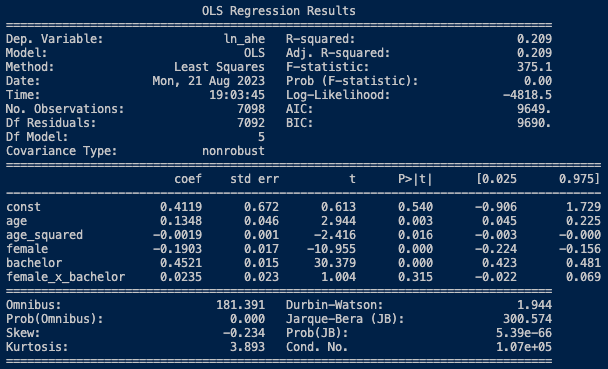
\includegraphics[width=0.80\textwidth]{final-exam-h-1.png}
          \end{figure}
          which is equivalent to the following linear regression equation:
          \begin{align*}
              \ln{(ahe)} & = &  & \beta_0 + \beta_1 (age) + \beta_2 (age^2)                                  \\
                         &   &  & + \beta_3 (female) + \beta_4 (bachelor) + \beta_5 (female \times bachelor) \\
              \ln{(ahe)} & = &  & 0.4119 + 0.1348 (age) - 0.0019 (age^2)                                     \\
                         &   &  & - 0.1903 (female) + 0.4521 (bachelor) + 0.0235 (female \times bachelor)
          \end{align*}
          For Alexis, a 30-year-old female with a bachelor's degree, her $\ln{(ahe)}$ is as follows:
          \begin{align*}
              \ln{(ahe)} & = 0.4119 + 0.1348 (30) - 0.0019 (30^2) - 0.1903 (1) + 0.4521 (1) + 0.0235 (1 \times 1) \\
                         & = 0.4119 + 4.044 - 1.71 - 0.1903 + 0.4521 + 0.0235                                     \\
                         & = \boldsymbol{3.0312}
          \end{align*}
          For Jane, a 30-year-old female with a high school degree, her $\ln{(ahe)}$ is as follows:
          \begin{align*}
              \ln{(ahe)} & = 0.4119 + 0.1348 (30) - 0.0019 (30^2) - 0.1903 (1) + 0.4521 (0) + 0.0235 (1 \times 0) \\
                         & = 0.4119 + 4.044 - 1.71 - 0.1903 + 0 + 0                                               \\
                         & = \boldsymbol{2.5556}
          \end{align*}
          The predicted difference between Alexis's and Jane's earnings is as follows:
          \begin{align*}
              e^{\ln{{(ahe)}_{Alexis}}} - e^{\ln{{(ahe)}_{Jane}}} & = e^{3.0312} - e^{2.5556} \\
                                                                  & = 20.7221 - 12.8790       \\
                                                                  & = \boldsymbol{7.8431}     \\
          \end{align*}
          For Bob, a 30-year-old male with a bachelor's degree, his $\ln{(ahe)}$ is as follows:
          \begin{align*}
              \ln{(ahe)} & = 0.4119 + 0.1348 (30) - 0.0019 (30^2) - 0.1903 (0) + 0.4521 (1) + 0.0235 (0 \times 1) \\
                         & = 0.4119 + 4.044 - 1.71 - 0 + 0.4521 + 0                                               \\
                         & = \boldsymbol{3.198}
          \end{align*}
          For Jim, a 30-year-old male with a high school degree, his $ln(ahe)$ is as follows:
          \begin{align*}
              \ln{(ahe)} & = 0.4119 + 0.1348 (30) - 0.0019 (30^2) - 0.1903 (0) + 0.4521 (0) + 0.0235 (0 \times 0) \\
                         & = 0.4119 + 4.044 - 1.71 - 0 + 0 + 0                                                    \\
                         & = \boldsymbol{2.7459}
          \end{align*}    The predicted difference between Bob's and Jim's earnings is as follows:
          \begin{align*}
              e^{\ln{{(ahe)}_{Alexis}}} - e^{\ln{{(ahe)}_{Jane}}} & = e^{3.198} - e^{2.7459} \\
                                                                  & = 24.4835 - 15.5786      \\
                                                                  & = \boldsymbol{8.9049}
          \end{align*}
          %%%%%%%%%%%%%%%%%%%%%%%%%%%%%%%%%%%%%%%%%%%%%%%%%%%%%%%%%%%%%%%%%%%%%%%%%%%%%%%%%%%%%%%%%%%%%%%%%%%%    
          %%%%%%%%%%%%%%%%%%%%%%%%%%%%%%%%%%%%%%%%%%%%%%%%%%%%%%%%%%%%%%%%%%%%%%%%%%%%%%%%%%%%%%%%%%%%%%%%%%%%    
          %%%%%%%%%%%%%%%%%%%%%%%%%%%%%%%%%%%%%%%%%%%%%%%%%%%%%%%%%%%%%%%%%%%%%%%%%%%%%%%%%%%%%%%%%%%%%%%%%%%%    
          %%%%%%%%%%%%%%%%%%%%%%%%%%%%%%%%%%%%%%%%%%%%%%%%%%%%%%%%%%%%%%%%%%%%%%%%%%%%%%%%%%%%%%%%%%%%%%%%%%%%    
          %%%%%%%%%%%%%%%%%%%%%%%%%%%%%%%%%%%%%%%%%%%%%%%%%%%%%%%%%%%%%%%%%%%%%%%%%%%%%%%%%%%%%%%%%%%%%%%%%%%%
    \item[i.] Is the effect of age on earnings different for men than for women? Specify
        and estimate a regression that you can use to answer this question. \\
        \textbf{Solution:} \\ We run a regression of $\ln{(ahe)}$ on $age, age^2,
            bachelor, age \times female$ in Python and obtain the following results, we
        skipped $female$ because it is not statistically significant:
        \begin{figure}[H]
            \centering
            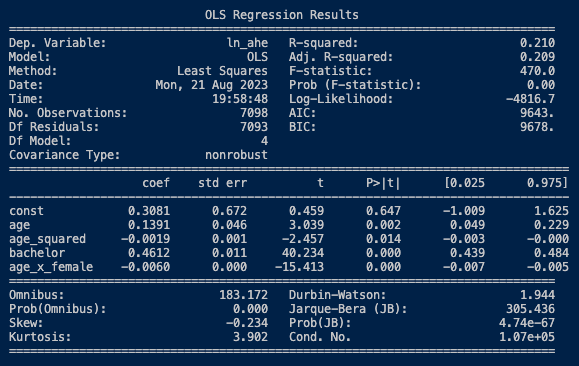
\includegraphics[width=0.80\textwidth]{final-exam-i-1.png}
        \end{figure}
        which is equivalent to the following linear regression equation:
        \begin{align*}
            \ln{(ahe)} & = \beta_0 + \beta_1 (age) + \beta_2 (age^2) + \beta_3 (bachelor) + \beta_4 (age \times female) \\
            \ln{(ahe)} & = 0.3081 + 0.1391 (age) - 0.0019 (age^2) + 0.4612 (bachelor) - 0.006(age \times female)
        \end{align*}
        $\beta_4 = -0.006$ represents the difference in the effect of age on earning for female compared to male,
        the negative sign indicates that the effect is less for female than for male. \\
        For example, all else equal, a 30-year-old male is expected to earn $e^{0.006 \times 30} = 119.7217\%$
        of a 30-year-old female.
        %%%%%%%%%%%%%%%%%%%%%%%%%%%%%%%%%%%%%%%%%%%%%%%%%%%%%%%%%%%%%%%%%%%%%%%%%%%%%%%%%%%%%%%%%%%%%%%%%%%%    
        %%%%%%%%%%%%%%%%%%%%%%%%%%%%%%%%%%%%%%%%%%%%%%%%%%%%%%%%%%%%%%%%%%%%%%%%%%%%%%%%%%%%%%%%%%%%%%%%%%%%    
        %%%%%%%%%%%%%%%%%%%%%%%%%%%%%%%%%%%%%%%%%%%%%%%%%%%%%%%%%%%%%%%%%%%%%%%%%%%%%%%%%%%%%%%%%%%%%%%%%%%%    
        %%%%%%%%%%%%%%%%%%%%%%%%%%%%%%%%%%%%%%%%%%%%%%%%%%%%%%%%%%%%%%%%%%%%%%%%%%%%%%%%%%%%%%%%%%%%%%%%%%%%    
        %%%%%%%%%%%%%%%%%%%%%%%%%%%%%%%%%%%%%%%%%%%%%%%%%%%%%%%%%%%%%%%%%%%%%%%%%%%%%%%%%%%%%%%%%%%%%%%%%%%%
    \item[j.] Is the effect of age on earnings different for high school graduates than
        for college graduates? Specify and estimate a regression that you can use to
        answer this question.\\ \textbf{Solution:} \\ We run a regression of
        $\ln{(ahe)}$ on $age, age^2, female, age \times bachelor$ in Python and obtain
        the following results, we skipped $bachelor$ because it will make $age \times
            bachelor$ statistically insiginficant.
        \begin{figure}[H]
            \centering
            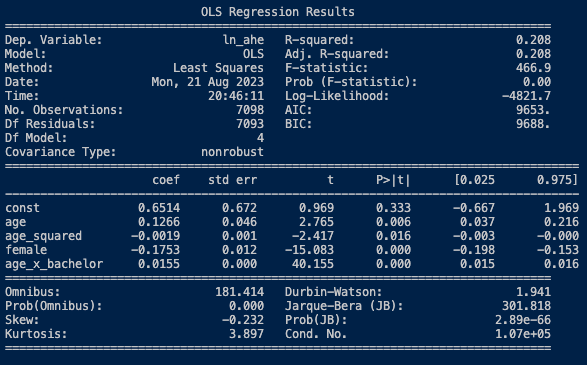
\includegraphics[width=0.80\textwidth]{final-exam-j-1.png}
        \end{figure}
        which is equivalent to the following linear regression equation:
        \begin{align*}
            \ln{(ahe)} & = \beta_0 +\beta_1(age) + \beta_2(age^2) + \beta_3(female) + \beta_4(age \times bachelor) \\
            \ln{(ahe)} & = 0.6514 + 0.1266(age) - 0.0019(age^2) -0.1753(female) + 0.0155(age \times bachelor)
        \end{align*}
        $\beta_4 = 0.0155$ represents the difference in the effect of age on earning for bachelor's degree holders,
        the positive sign indicates that the effect is more for bachelor's degree holders. \\
        For example, all else equal, a 30-year-old bachelor's degree holder is expected to earn $e^{0.0155 \times 30} = 159.2014\%$
        of a high school degree holder.
        %%%%%%%%%%%%%%%%%%%%%%%%%%%%%%%%%%%%%%%%%%%%%%%%%%%%%%%%%%%%%%%%%%%%%%%%%%%%%%%%%%%%%%%%%%%%%%%%%%%%    
        %%%%%%%%%%%%%%%%%%%%%%%%%%%%%%%%%%%%%%%%%%%%%%%%%%%%%%%%%%%%%%%%%%%%%%%%%%%%%%%%%%%%%%%%%%%%%%%%%%%%    
        %%%%%%%%%%%%%%%%%%%%%%%%%%%%%%%%%%%%%%%%%%%%%%%%%%%%%%%%%%%%%%%%%%%%%%%%%%%%%%%%%%%%%%%%%%%%%%%%%%%%    
        %%%%%%%%%%%%%%%%%%%%%%%%%%%%%%%%%%%%%%%%%%%%%%%%%%%%%%%%%%%%%%%%%%%%%%%%%%%%%%%%%%%%%%%%%%%%%%%%%%%%    
        %%%%%%%%%%%%%%%%%%%%%%%%%%%%%%%%%%%%%%%%%%%%%%%%%%%%%%%%%%%%%%%%%%%%%%%%%%%%%%%%%%%%%%%%%%%%%%%%%%%%
    \item[k.] After running all these regressions, summarize the effect of age on
        earnings for young workers.\\ \textbf{Solution:}\\ All regressions have
        consistently shown that the effect of $age$ on $ahe$ is positive. However, by
        running the regression of $\ln{ahe}$ on $age, age^2$, the model suggests that
        the positive effect of $age$ on $ahe$ is decreasing and eventually plateaus.
        $bachelor$ showed a very strong positive effect on $ahe$ and $female$ showed a
        negative effect on $ahe$. \newpage

    \item[] \textbf{Extra Credit:} \\
        Although the assignment refers to a single source of data, there are 7 different regression models
        from (a), (b), (c), (d), (h), (i), and (j).  \\
        Besides, having extremely hand-on experiece with applying models and reading results, we also learnt
        that understanding the nature of the data is very important. For example, if we did not take
        into consideration the diminishing effect of age on earnings, we would have concluded that
        the effect of age on earnings is positive and increasing linearly forever, which is pretty absurd. \\
        Also, linking from project 1, 2 to this final exam, I noticed that the way I used Python code for 
        modeling and analyzing data has improved, I am very comfortable using Python stats, numpy to do 
        regression after this series of problems. \\
\end{enumerate}

\begin{python}
# All related code for the assignment is below:
import numpy as np
import statsmodels.api as sm
import pandas as pd


class CurrentPopulationSurveyDataFrame:
    df = None

    def __init__(self):
        file_path = 'CPS2015-1.xlsx'
        file_sheet_name = 'Data'
        self.df = pd.read_excel(file_path, sheet_name=file_sheet_name)


def part_a():
    df = CurrentPopulationSurveyDataFrame().df
    Y = df['ahe']
    X = df[['age', 'female', 'bachelor']]
    X = sm.add_constant(X)
    model = sm.OLS(Y, X).fit()
    print()
    print(model.summary())


def part_b():
    df = CurrentPopulationSurveyDataFrame().df
    df['ln_ahe'] = np.log(df['ahe'])
    Y = df['ln_ahe']
    X = df[['age', 'female', 'bachelor']]
    X = sm.add_constant(X)
    model = sm.OLS(Y, X).fit()
    print()
    print(model.summary())


def part_c():
    df = CurrentPopulationSurveyDataFrame().df
    df['ln_ahe'] = np.log(df['ahe'])
    df['ln_age'] = np.log(df['age'])
    Y = df['ln_ahe']
    X = df[['ln_age', 'female', 'bachelor']]
    X = sm.add_constant(X)
    model = sm.OLS(Y, X).fit()
    print()
    print(model.summary())


def part_d():
    df = CurrentPopulationSurveyDataFrame().df
    df['ln_ahe'] = np.log(df['ahe'])
    df['age_squared'] = np.square(df['age'])
    Y = df['ln_ahe']
    X = df[['age', 'age_squared', 'female', 'bachelor']]
    X = sm.add_constant(X)
    model = sm.OLS(Y, X).fit()
    print()
    print(model.summary())


def part_e():
    df = CurrentPopulationSurveyDataFrame().df
    df['ln_ahe'] = np.log(df['ahe'])
    df['age_squared'] = np.square(df['age'])
    df['female_x_bachelor'] = df['female'] * df['bachelor']
    Y = df['ln_ahe']
    X = df[['age', 'age_squared', 'female', 'bachelor', 'female_x_bachelor']]
    X = sm.add_constant(X)
    model = sm.OLS(Y, X).fit()
    print()
    print(model.summary())


def part_i():
    df = CurrentPopulationSurveyDataFrame().df
    df['ln_ahe'] = np.log(df['ahe'])
    df['age_squared'] = np.square(df['age'])
    df['age_x_female'] = df['age'] * df['female']
    Y = df['ln_ahe']
    X = df[['age', 'age_squared', 'bachelor', 'age_x_female']]
    X = sm.add_constant(X)
    model = sm.OLS(Y, X).fit()
    print()
    print(model.summary())


def part_j():
    df = CurrentPopulationSurveyDataFrame().df
    df['ln_ahe'] = np.log(df['ahe'])
    df['age_squared'] = np.square(df['age'])
    df['age_x_bachelor'] = df['age'] * df['bachelor']
    Y = df['ln_ahe']
    X = df[['age', 'age_squared', 'female', 'age_x_bachelor']]
    X = sm.add_constant(X)
    model = sm.OLS(Y, X).fit()
    print()
    print(model.summary())


if __name__ == '__main__':
    part_j()

\end{python}
%%%%%%%%%%%%%%%%%%%%%%%%%%%%%%%%%%%%%%%%%%%%%%%%%%%%%%%%%%%%%%%%%%%%%%%%%%%%%%%%%%%%%%%%%%%%%%%%%%%%    
\end{document}